\documentclass[10pt]{beamer}

\usetheme[progressbar=frametitle]{metropolis}
\usepackage{appendixnumberbeamer}


\usepackage{array,booktabs}
\usepackage[scale=2]{ccicons}
\usepackage{multicol}
\usepackage{mathtools}
\usepackage{array}

\usepackage{pgfplots}
\usepgfplotslibrary{dateplot}

\usepackage{xspace}
\newcommand{\themename}{\textbf{\textsc{metropolis}}\xspace}
\let\oldfootnotesize\footnotesize
\renewcommand*{\footnotesize}{\oldfootnotesize\tiny}
\let\oldabs\abs
\def\abs{\@ifstar{\oldabs}{\oldabs*}}


\title{Evaluation metrics matter: predicting sentiment from financial news headlines.}
\author{Andrew Moore and Paul Rayson}
\date{\today}
\institute{School of Computing and Communications, Lancaster University.}
\titlegraphic{\hfill
\includegraphics[height=1.5cm]{ucrel_logo_2016.png}}

\begin{document}

\maketitle

\begin{frame}{Table of contents}
  \setbeamertemplate{section in toc}[sections numbered]
  \tableofcontents[hideallsubsections]
\end{frame}

\section{Introduction}

\begin{frame}[fragile]{What is SemEval}
  \begin{figure}
    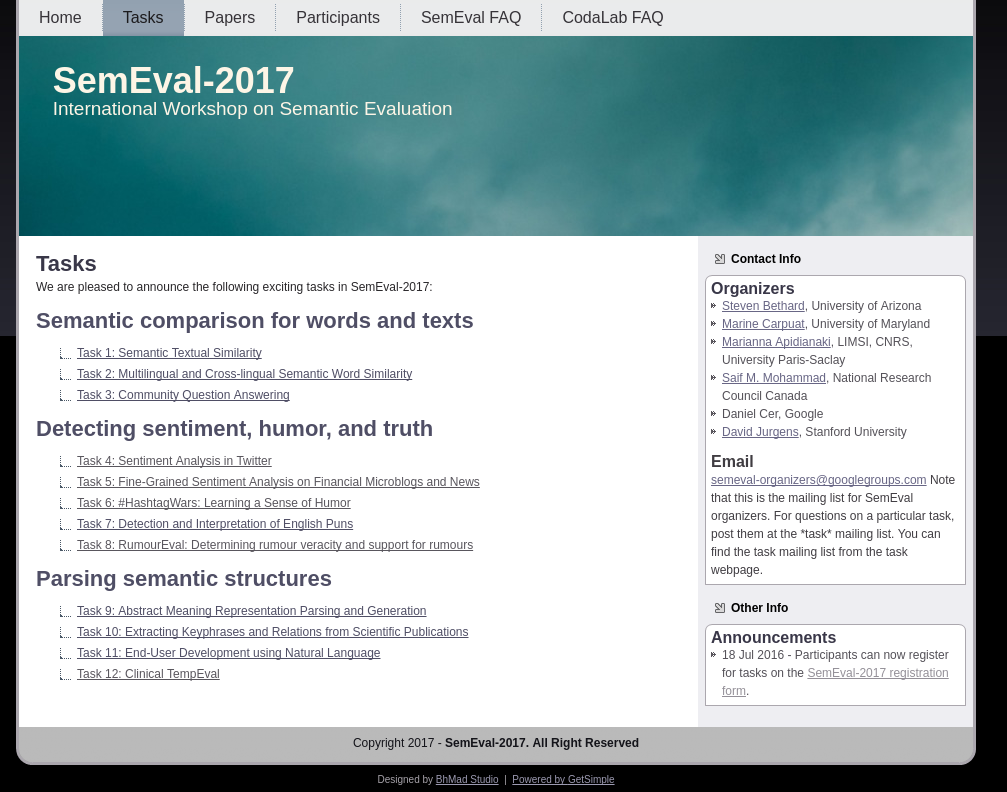
\includegraphics[scale=0.3]{SemEval.png}
  \end{figure}
\end{frame}

% Given a financial headline that has come from different sources on the 
% internet such as Yahoo finance. Predict the sentiment of the headline 
% with respect to a company for example here there are two comapnies here 
% therefore two sentiments will have to be predicted one for Dixons 
% and one for AstrZeneca. The sentiment to be predicted ranges from -1
% to 1 where 1 is positive and -1 negative and 0 being neutral.

\begin{frame}[fragile]{The task}
\begin{block}{Example sentence}
\begin{center}
`Why \alert{AstraZeneca plc} \& \alert{Dixons Carphone PLC} Are Red-Hot Growth Stars!'
\end{center}
\end{block}

\begin{block}{Sentiment scale}
\begin{figure}
    
\includegraphics[scale=0.3]{sentiment_range.png}
  \end{figure}
\end{block}

\begin{block}{Data}
Training data: 1142 samples, 960 headlines/sentences.\newline
Testing data: 491 samples, 461 headlines/sentences.
\end{block}

\end{frame}

\begin{frame}[fragile]{Evaluation metric}
% They gave us a dataset of 1142 training examples and we were evaluated on 491 test examples. The metric used to determine our accuracy was cosine similarity. As you can see it takes two vectors of values one being the predicted sentiment and the other being the true correct values and the metric finds how close the predicted sentiments are to the correct as you can see from the example. 
\begin{block}{Cosine Similarity (CS) \footnote{Taken from Wikipedia \url{https://en.wikipedia.org/wiki/Cosine_similarity}}}
\begin{equation}
\frac{ \sum\limits_{i=1}^{K}{A_i  B_i} }{ \sqrt{\sum\limits_{i=1}^{K}{A_i^2}}  \sqrt{\sum\limits_{i=1}^{K}{B_i^2}} }
\end{equation}
\end{block}

\begin{block}{Example}
\textit{A} = Predicted sentiment = [0.5, -0.2] \newline
\textit{B} = True sentiment = [0.4, 0.1] \newline 
Cosine similarity = 0.189
\end{block}

\end{frame}

\section{Approach}
\begin{frame}[fragile]{Additional data used}

\begin{block}{Word2Vec model}
Used 189, 206 financial articles (e.g. Financial Times) that were manually downloaded from Factiva\footnote{\url{https://global.factiva.com/factivalogin/login.asp?productname=global}} to create a Word2Vec model \cite{mikolov2013efficient}\footnote{\url{https://github.com/apmoore1/semeval/tree/master/models/word2vec_models}}.\newline\newline
These were created using Gensim\footnote{\url{https://radimrehurek.com/gensim/models/word2vec.html}}.
\end{block}

\end{frame}

\begin{frame}[fragile]{Support Vector Regression (SVR) \cite{drucker1997support}}
\begin{block}{Features and settings that we changed}
\begin{enumerate}
\item Tokenisation - Whitespace or Unitok\footnote{\url{http://corpus.tools/wiki/Unitok}}
\item N-grams - uni-grams, bi-grams and both.
% These define how generalisable the SVR is higher the eplison value the more general as a value in the training dataset won't have such a large affect on the algorithm and the lower the C value the larger the margin and the more generalisable. 
\item SVR settings - penalty parameter C and epsilon parameter.
\item Target aspect. 
\item Word Replacements.
\end{enumerate}

\end{block}

\end{frame}

\begin{frame}[fragile]{Word Replacements}
% This was based mainly on intuition that we did not have enough training data to accurately predict the sentiment therefore I thought we should try and reduce the sparsity problem that a Bag of words approach causes by replacing certain words with affectively a form of semantic tag. The company name was found using the list of company names provided from the data and the positive and negative words were found by using the N most similar words that were most similar to the words Excellent and poor.
\begin{block}{Example Sentence}
`\textcolor{green}{AstraZeneca PLC} had an \textcolor{blue}{improved} performance where as \textcolor{green}{Dixons} performed \textcolor{red}{poorly}'\newline\newline
`\textcolor{green}{companyname} had an \textcolor{blue}{posword} performance where as \textcolor{green}{companyname} performed \textcolor{red}{negword}'
\end{block}

\end{frame}

\begin{frame}[fragile]{Word Replacements}
\begin{block}{Company example N=10 company = `tesco'}
\begin{multicols}{2}
\begin{description}
\item [sainsbury] 0.6729
\item [asda] 0.5999
\item [morrisons] 0.5188
\item [supermarkets] 0.5089
\item [kingfisher] 0.4956
\item [primark] 0.4811
\item [grocer] 0.4792
\item [unilever] 0.4764
\item [wal-mart] 0.4750
\item [waitrose] 0.4713
\end{description}
\end{multicols}

\end{block}

\end{frame}

\begin{frame}[fragile]{Bi-directional Long Short-Term Memory BLSTM \cite{graves2005framewise}\cite{hochreiter1997long}}
\begin{figure}
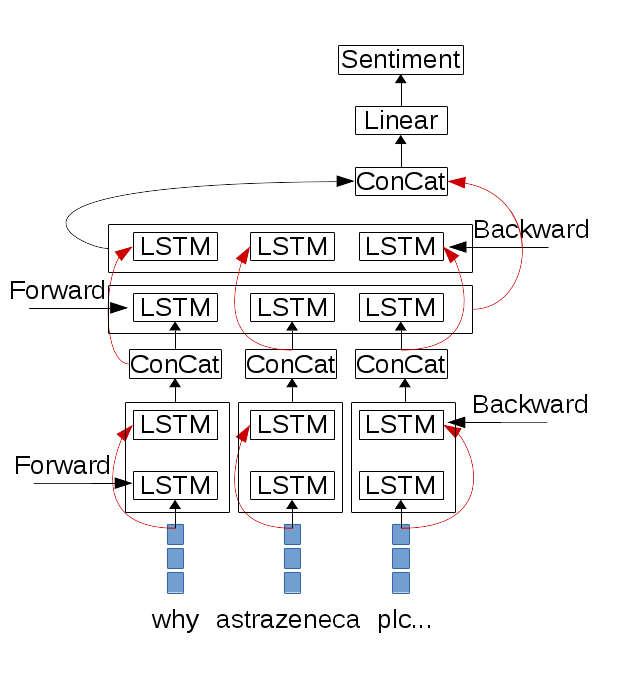
\includegraphics[scale=0.3]{lstm_diagram.png}
\end{figure}
\end{frame}

\begin{frame}[fragile]{BLSTM Sentence representation}
\begin{enumerate}
\item Sentences are fixed length.
\item All words are represented as vectors.
\end{enumerate}
\begin{block}{Example}
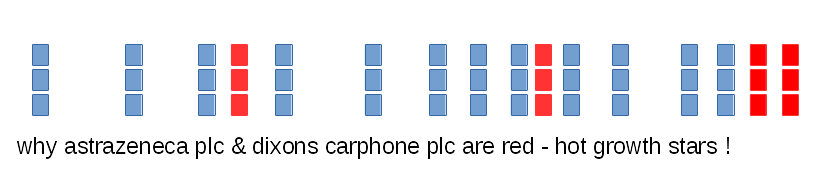
\includegraphics[scale=0.4]{sentence_rep.png}
\end{block}

\end{frame}

\begin{frame}[fragile]{BLSTM LSTM network\footnote{Image idea taken from: \url{https://colah.github.io/posts/2015-08-Understanding-LSTMs/}}}
\begin{columns}[T,onlytextwidth]
    \column{0.6\textwidth}
    \begin{block}{LSTM network}
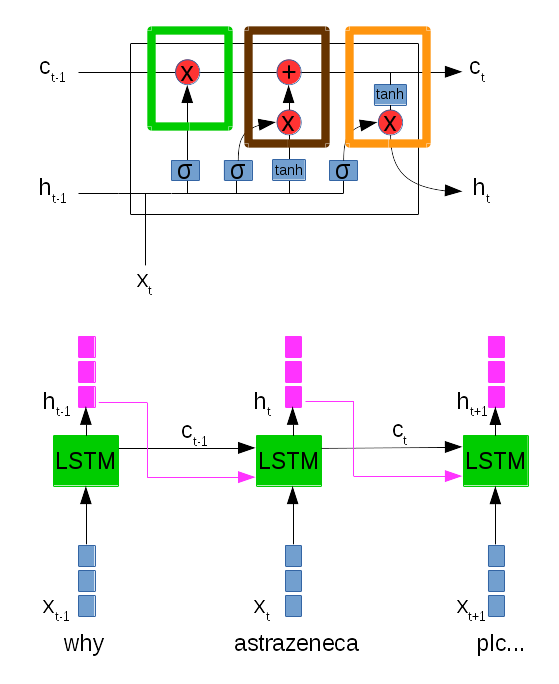
\includegraphics[scale=0.3]{lstm_network.png}
\end{block}

    \column{0.4\textwidth}

      \begin{block}{Properties}
        \begin{enumerate}
        \item \textbf{\textcolor{green}{Forgot gate.}}
        \item \textbf{\textcolor{brown}{Input gate.}}
        \item \textbf{\textcolor{orange}{Output gate.}}
        \end{enumerate}
      \end{block}

  \end{columns}
\end{frame}
\begin{frame}[fragile]{BLSTM LSTM network}
\begin{block}{The advantages of LSTMs}
\begin{enumerate}
\item Good at learning sequential data.
\item Able to learn long term dependencies.
\end{enumerate}

\end{block}
\begin{block}{LSTM related work}
\begin{enumerate}
\item Google have improved their translation system using LSTMs\cite{wu2016google}
\item  Chiu and Nichols improved Named Entity Recognition\cite{chiu2015named}.
\end{enumerate}

\end{block}

\end{frame}

\begin{frame}[fragile]{BLSTM architecture explained}
\begin{columns}[T,onlytextwidth]
\column{0.6\textwidth}
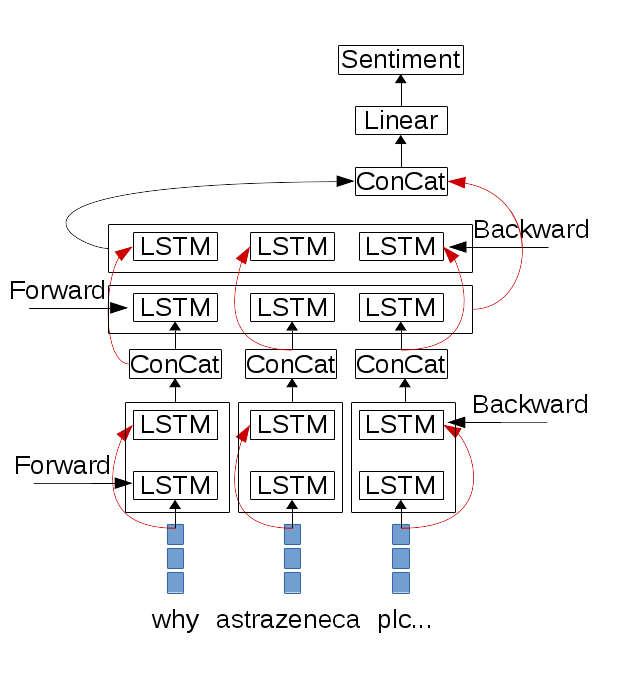
\includegraphics[scale=0.3]{lstm_diagram.png}

\column{0.4\textwidth}
\centering
\begin{block}{Loss function\newline Mean Square Error (MSE)}
\begin{equation}
\frac{1}{Y}\sum\limits_{i=1}^{Y} (\hat y_i - y)^2
\end{equation}

\end{block}
\end{columns}
\end{frame}

\begin{frame}[fragile]{Two BLSTM models}
\begin{columns}[T,onlytextwidth]
    \column{0.6\textwidth}
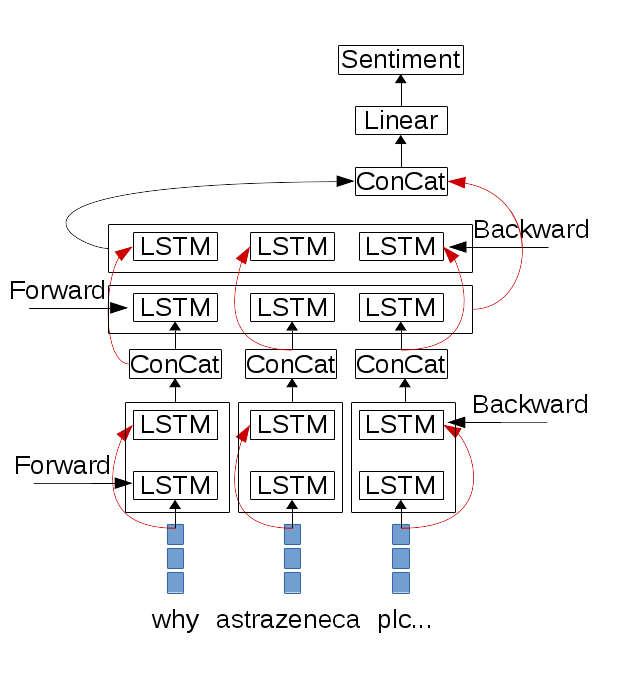
\includegraphics[scale=0.3]{lstm_diagram.png}

    \column{0.4\textwidth}

      \begin{block}{Standard Model (SLSTM)}
\begin{itemize}
\item Drop out between layers and connections.
\item 25 times trained over the data (epoch of 25).
\end{itemize}

\end{block}
\begin{block}{Early stopping model (ELSTM)}
\begin{itemize}
\item Drop out between layers only.
\item Early stopping used to determine the epoch.
\end{itemize}

\end{block}

  \end{columns}


\end{frame}

\section{Findings and Results}

\begin{frame}[fragile]{SVR best features}
\begin{block}{Features}
\begin{itemize}
\item Using uni-grams and bi-grams to be the best.
\item Using a tokeniser always better. Affects bi-gram results the most.
\item SVR parameter settings important 8\% difference between using C=0.1 and C=0.01. 
\item Incorporating the target aspect increased performance.
\item Using all word replacements. N=10 for pos and neg words and N=0 for company.
\end{itemize}
\end{block}

\end{frame}

\begin{frame}[fragile]{Results}

\begin{columns}[T,onlytextwidth]
\column{0.33\textwidth}
\begin{block}{SVR}
60.21\%
\end{block}
\column{0.33\textwidth}
\begin{block}{SLSTM}
73.20\%
\end{block}
\column{0.33\textwidth}
\begin{block}{ELSTM}
73.27\%
\end{block}

\end{columns}


\end{frame}
\begin{frame}[fragile]{Future Work}
\begin{columns}[T,onlytextwidth]
    \column{0.6\textwidth}
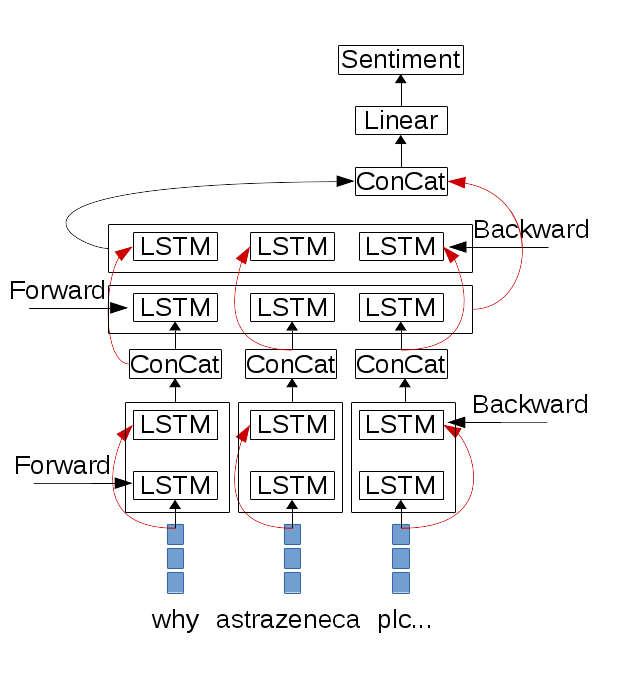
\includegraphics[scale=0.3]{lstm_diagram.png}

    \column{0.4\textwidth}
\begin{enumerate}
\item Incorporate aspects into the BLSTM's shown to be useful by Wang et al. \cite{wangattention}.
\item Improve BLSTM's by using an attention model Wang et al. \cite{wangattention}.
\end{enumerate}
\end{columns}
\end{frame}

\begin{frame}[fragile]{Future Work}
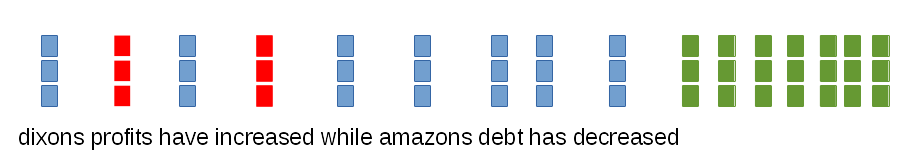
\includegraphics[scale=0.3]{sentence_attention.png}

\begin{enumerate}
\item Incorporate aspects into the BLSTM's shown to be useful by Wang et al. \cite{wangattention}.
\item Improve BLSTM's by using an attention model Wang et al. \cite{wangattention}.
\end{enumerate}

\end{frame}

\section{Why evaluation metrics matter}

\begin{frame}[fragile]{The task}
`given a text instance predict the sentiment score for each of the companies/stocks mentioned'\footnote{\url{http://alt.qcri.org/semeval2017/task5/}}

\end{frame}


\begin{frame}[fragile]{The three different metrics}

\begin{columns}[T,onlytextwidth]

\column{0.33\textwidth}
\begin{block}{Cosine Similarity (CS) Metric 1}
\begin{equation}
\frac{ \sum\limits_{i=1}^{K}{y_i  \hat y_i} }{ \sqrt{\sum\limits_{i=1}^{K}{y_i^2}}  \sqrt{\sum\limits_{i=1}^{K}{\hat y_i^2}} }
\end{equation}
\end{block}

\column{0.66\textwidth}
\begin{block}{Metric 2}
\begin{equation}
\label{eq:first_eval}
\begin{gathered}
\frac{\sum_{n=1}^{N} \text{CS}(\hat y_n, y_n)}{N}
\end{gathered}
\end{equation}
\end{block}

\begin{block}{Metric 3}
\begin{equation}
\begin{gathered}
\frac{\sum_{n=1}^{N} \begin{cases}len(\hat y_n) * \text{CS}(\hat y_n, y_n), & \text{if}\ len(\hat y_n) > 1 \\
      1 - \lvert y - \hat y_n \rvert, & \text{if}\ \frac{\hat y_n}{y}\geq0
      \end{cases} }{K}
\end{gathered}
\end{equation}

\end{block}

\end{columns}
\textit{K} = Total number of samples. \newline
\textit{N} = Total number of sentences.


\end{frame}

\begin{frame}[fragile]{The differences in metrics\footnote{Code for this slide \url{https://github.com/apmoore1/semeval/blob/master/examples/metric_examples.py}}}
\begin{table}[c]
\centering
\label{my-label}
\begin{tabular}{cccccc}
 \multicolumn{2}{c}{} & \multicolumn{3}{c}{Metric} & \multicolumn{1}{c}{} \\
 \cmidrule(lr){3-5} 
 PS& TS&  1&  2&  3& No. Sentences\\
 $[$$[$0.2$]$,$[$0.5$]$$]$&  $[$$[$-0.4$]$,$[$-0.1$]$$]$&  -0.585&  -1&  0&  2\\
$[$$[$0.9$]$,$[$0.2$]$$]$&  $[$$[$0.8$]$,$[$0.3$]$$]$&  0.99&  1&  0.9&  2\\
 $[$$[$0.2, 0.3$]$$]$&  $[$$[$-0.1, -0.2$]$$]$&  -0.992&  -0.496&  -0.992& 1
\end{tabular}
\end{table}
PS = Predicted Sentiment \newline
TS = True Sentiment \newline \newline
All of the above are two samples.

\end{frame}

\begin{frame}[fragile]{Different metrics different results \footnote{code this slide \url{https://github.com/apmoore1/semeval/blob/master/examples/run.py}}}
\begin{table}[c]
\centering
\begin{tabular}{cccc}
 \multicolumn{1}{c}{} & \multicolumn{3}{c}{Metric} \\
 Model&  1&  2&  3 \\
 SVR&  62.14&  54.59&  62.34 \\
 SLSTM&  72.89&  61.55&  68.64 \\
 ELSTM&  73.20&  61.98&  69.24 
 
\end{tabular}
\end{table}
\end{frame}

\begin{frame}[fragile]{Metrics should reflect the problem}
\begin{block}{Problem}
To identify `bullish (optimistic; believing that the stock price will increase) and bearish (pessimistic; believing that the stock price will decline) sentiment associated with companies and stocks.'\footnote{http://alt.qcri.org/semeval2017/task5/}
\end{block}

\begin{block}{Main reason against metric 1}
That scores with opposite sentiment should not be rewarded in any way.
\end{block}

\end{frame}

\begin{frame}[fragile]{Recomended blog posts for word vectors}
\begin{enumerate}
\item \url{https://colah.github.io/posts/2014-07-NLP-RNNs-Representations/}
\item \url{http://sebastianruder.com/word-embeddings-1/}
\end{enumerate}

\end{frame}

\begin{frame}[fragile]{Recomended blog posts for RNN/LSTM}
\begin{enumerate}
\item \url{https://deeplearning4j.org/lstm} - Good place to start.
\item \url{https://colah.github.io/posts/2015-08-Understanding-LSTMs/} - Good place to understand LSTM.
\item \url{https://karpathy.github.io/2015/05/21/rnn-effectiveness/} on the applications of RNN's.
\item \url{https://skillsmatter.com/skillscasts/6611-visualizing-and-understanding-recurrent-networks} video on RNN's.\footnote{14.44 mins tips on how to train RNN/LSTM architectures.}
\item \url{https://nbviewer.ipython.org/gist/yoavg/d76121dfde2618422139} usefulness of RNN's.
\end{enumerate}

\end{frame}

\begin{frame}[fragile]{Other related resources}
\begin{enumerate}
\item Recommended book - \url{http://www.deeplearningbook.org/}
\item Oxford Deep learning course - \url{https://github.com/oxford-cs-deepnlp-2017/lectures}
\item Stanford courses
\begin{enumerate}
\item Machine Learning - CS229
\item NLP with deep learning - CS224n 
\item CNN for visual recognition - CS231n
\end{enumerate}

\end{enumerate}

\end{frame}

\begin{frame}[fragile]{Drawings to code}
\begin{figure}
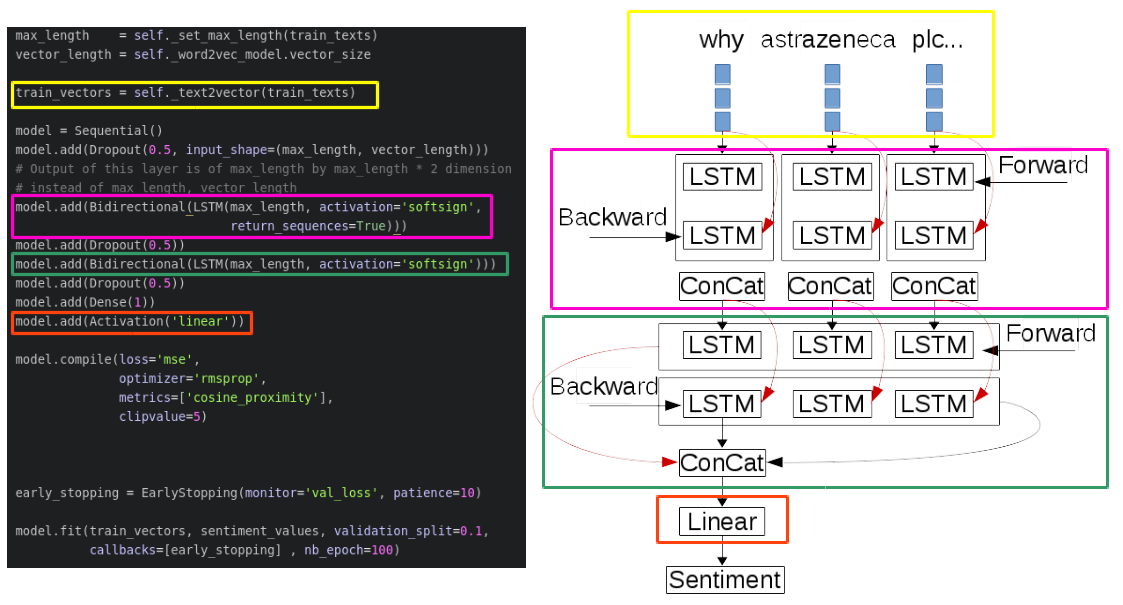
\includegraphics[scale=0.3]{lstm_code_to_diagram.png}
\end{figure}
\end{frame}

\begin{frame}[fragile]{Python libraries used}
\begin{enumerate}
\item Scikit-learn for the SVR - \url{http://scikit-learn.org/stable/}
\item Keras for the BLSTMs - \url{https://keras.io/}
\end{enumerate}

\end{frame}

\begin{frame}[fragile]{Summary}
\begin{enumerate}
\item BLSTM outperform SVRs with minimal feature engineering.
\item Define your evaluation metric with regards to your real world problem.
\item Ensure that you know your evaluation metric before creating your system.
\end{enumerate}

\end{frame}

\begin{frame}[plain]
\begin{center}
\begin{center}
\huge Questions?
\end{center}
\begin{center}
\begin{columns}[T,onlytextwidth]
\column{0.1\textwidth}
\column{0.4\textwidth}
\centering
\normalsize a.moore@lancaster.ac.uk
\column{0.4\textwidth}
\centering
\normalsize @apmoore94
\column{0.1\textwidth}
\end{columns}
\end{center}
\end{center}

\begin{center}
\begin{center}
\small All the code can be found here\footnote{\url{https://github.com/apmoore1/semeval}}
\end{center}
\begin{center}
\small Presentation can be found here \footnote{\url{https://github.com/apmoore1/semeval/blob/master/presentation/slides.pdf}}
\end{center}
\end{center}

\end{frame}




\begin{frame}[allowframebreaks]{References}
  \bibliography{demo}
  \bibliographystyle{abbrv}

\end{frame}

\end{document}
